\documentclass[a4paper,12pt]{article}
\usepackage{karnaugh-map}
\usepackage[utf8]{inputenc}
\usepackage{amssymb,amsmath}
\usepackage{float}
\usetikzlibrary{arrows, shapes.gates.logic.US, calc}
\tikzstyle{branch}=[fill, shape=circle, minimum size=3pt, inner sep=0pt]
    
\begin{document}

\section*{Task 3: Issues at minimal cost implementation}

Given a truth table, it was requested to see what happens
when the truth table is implemented with the smallest quantity of logic
gates. To perform this task, ICs that either have NOR 
or NAND logic gates will be used.

\subsection*{Low cost approach}
\begin{figure}[htbp]
    \begin{center}
    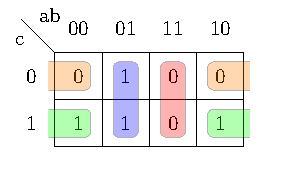
\includegraphics{karnaugh_test.pdf}
    \end{center}
    \caption{Karnaugh   Map of the given truth table}
    \end{figure} 
We can get the minimal cost output expressed either in groups of 
maxterms (orange and red groups) or minterms (blue and green groups).
\linebreak
Let Z be the output label, its maxterms expression is:
\begin{equation}
    Z= (\bar{A}.B)+(C.\bar{B})
\end{equation} 
Also, its minterms expression is:
\begin{equation}
    Z= (\bar{A}+\bar{B}).(C+B)
\end{equation} 
\begin{figure}[htbp]
    \begin{center}
        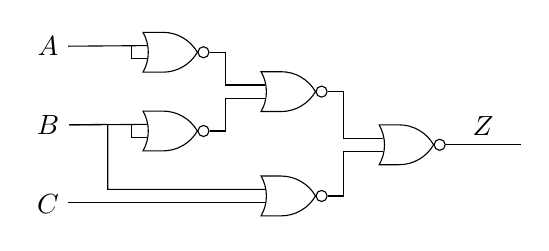
\begin{tikzpicture}
            %seteamos el orden de las variables
            \node (x) at (0, 2)(x) {$A$};
            \node (y) at (0, 1) (y){$B$};
            \node (z) at (0, 0)(z) {$C$};
        
            %creamos un nodo con una posicion asociada:($(x)) que es donde se encuentra
            %posicionada la variable x y le ponemos nombre: nor_x
            %los numeros son para desplazar la compuertas
            \node[nor gate US, draw, rotate=0, logic gate inputs=nn] at ($(x) + (1.5, -0.075)$) (nor_x) {};
            \node[nor gate US, draw, rotate=0, logic gate inputs=nn] at ($(y) + (1.5, -0.075)$) (nor_y) {};
            
            %dibujar la nor con las entradas unidas:
            %primero dibujamos una linea
            \draw (x) -- (nor_x.input 1); 
            % ahora dibujamos desplazada la linea que va a entrar al input 2
            \draw (nor_x.input 2) -- ([xshift=-0.2cm]nor_x.input 2) |- (nor_x.input 1);
        
            \draw (y) -- (nor_y.input 1);
            \draw (nor_y.input 2) -- ([xshift=-0.2cm]nor_y.input 2) |- (nor_y.input 1);
        
            %asigno dos entradas
            \node[nor gate US, draw, rotate=0, logic gate inputs=nn] at ($(x) + (3, -0.075-0.5)$) (norAndB) {};
            \draw (nor_x.output) -- ([xshift=0.2cm]nor_x.output) |- (norAndB.input 1);
            \draw (nor_y.output) -- ([xshift=0.2cm]nor_y.output) |- (norAndB.input 2);
        
            \node[nor gate US, draw, rotate=0, logic gate inputs=nn] at ($(z) + (3, 0+0.10)$) (norBandC) {};
            \draw (z) -- ([xshift=0.2cm]z) |- (norBandC.input 2);
            \draw (y) -- ([xshift=-0.5cm]nor_y.input 1)  |- (norBandC.input 1);
        
            \node[nor gate US, draw, rotate=0, logic gate inputs=nn] at ($(y) + (4.5, -0.25)$) (norFinal) {};
            \draw (norAndB.output) -- ([xshift=0.2cm]norAndB.output) |- (norFinal.input 1);
            \draw (norBandC.output) -- ([xshift=0.2cm]norBandC.output) |- (norFinal.input 2);
        
            \draw (norFinal.output) -- node[above]{$Z$} ($(norFinal) + (1.5, 0)$);
        \end{tikzpicture}
        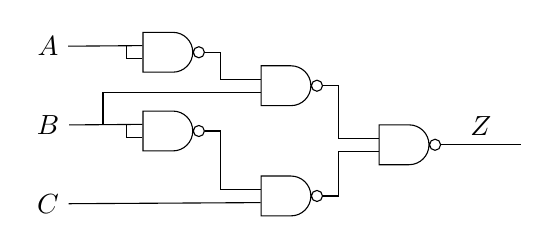
\begin{tikzpicture}
            \node (x) at (0, 2)(x) {$A$};
            \node (y) at (0, 1) (y){$B$};
            \node (z) at (0, 0)(z) {$C$};
            \node[nand gate US, draw, rotate=0, logic gate inputs=nn] at ($(x) + (1.5, -0.075)$) (nand_x) {};
            \draw (x) -- (nand_x.input 1); 
            \draw (nand_x.input 2) -- ([xshift=-0.2cm]nand_x.input 2) |- (nand_x.input 1);
            \node[nand gate US, draw, rotate=0, logic gate inputs=nn] at ($(x) + (3, -0.5)$) (nandAandB) {};
            \draw (nand_x.output) -- ([xshift=0.2cm]nand_x.output) |- (nandAandB.input 1);
            \node[nand gate US, draw, rotate=0, logic gate inputs=nn] at ($(y) + (1.5, -0.075)$) (nand_y) {};
            \draw (y) -- (nand_y.input 1); 
            \draw (nand_y.input 2) -- ([xshift=-0.2cm]nand_y.input 2) |- (nand_y.input 1);
            \draw (nand_y.input 1) -- ([yshift=0cm]nand_y.input 1) -- ([xshift=-0.5cm]nand_y.input 1) |- (nandAandB.input 2);
            \node[nand gate US, draw, rotate=0, logic gate inputs=nn] at ($(z) + (3,0.1)$) (nandBandC) {};
            \draw (z) -- (nandBandC.input 2); 
            \draw (nand_y.output) -- ([xshift=0.2cm]nand_y.output) |- (nandBandC.input 1);
            \node[nand gate US, draw, rotate=0, logic gate inputs=nn] at ($(y) + (4.5, -0.25)$) (nandFinal) {};
            \draw (nandAandB.output) -- ([xshift=0.2cm]nandAandB.output) |- (nandFinal.input 1);
            \draw (nandBandC.output) -- ([xshift=0.2cm]nandBandC.output) |- (nandFinal.input 2);
            \draw (nandFinal.output) -- node[above]{$Z$} ($(nandFinal) + (1.5, 0)$);

        \end{tikzpicture}



    \end{center}
    \caption{Implementation with NOR gates and NAND gates respectively}
\end{figure} 

Note that the quantity of logic gates in both cases are the same.

\section{Introduction}

Here is the text out your introduction.

\begin{equation}
    \label{simple_equation}
    \alpha = \sqrt{ \beta }
\end{equation}

\subsection{Subsection Heading Here}
Write your subsection text here.

\section{Conclusion}
Write your conclusion here.

\end{document}